\chapter{Exercices de fin de document (14 à 19)}

% ------------------------------------------------------------------
\section{Exercice 14 : température dans un mur}

\Attention À $t = 0$, la face $x = L$ est à $T_0$ (condition initiale) mais doit
être à $T_L$ (condition aux limites) : les deux conditions ne se raccordent
pas si $T_L \ne T_0$. On impose $T_L$ dès le premier nœud de temps
($T_{m,0} = T_L$) ; ce choix n'influe que sur les tout premiers pas. En $x = 0$,
$T_0 + T_1\sin 0 = T_0$ : pas de conflit. Le temps $t$ est mesuré dans l'unité
implicite de la loi $\sin(\pi t/2)$ (période 4).

\Question{1-a- Forme discrète par différences progressives.}
\Pourquoi C'est le schéma explicite du cours (C2) appliqué à
$\partial T/\partial t = \alpha\,\partial^2T/\partial x^2$ ; seules les conditions
aux limites changent.
\Etapes
\Etape{1} Grille $x_i = i\Delta x$, $\Delta x = L/m$ ; $t_j = j\Delta t$ ;
$T_{i,j} \approx T(x_i, t_j)$ ; $\lambda = \alpha\Delta t/\Delta x^2$.
\Etape{2} Dérivée en temps progressive, dérivée en espace centrée :
\[
  \frac{T_{i,j+1} - T_{i,j}}{\Delta t} = \alpha\,\frac{T_{i+1,j} - 2T_{i,j} + T_{i-1,j}}{\Delta x^2}
  \;\Longrightarrow\;
  T_{i,j+1} = \lambda T_{i+1,j} + (1 - 2\lambda)T_{i,j} + \lambda T_{i-1,j},
\]
pour $i = 1, \dots, m-1$ et $j \ge 0$.
\Etape{3} Conditions : $T_{i,0} = T_0$ ($0 \le i < m$), $T_{m,j} = T_L$,
$T_{0,j} = T_0 + T_1\sin(\pi j\Delta t/2)$.
\Etape{4} Erreur de discrétisation : $O(\Delta t)$ pour la dérivée en temps et
$O(\Delta x^2)$ pour la dérivée en espace, soit $O(\Delta t + \Delta x^2)$
\BF{p.~747}. Le schéma est stable si $\lambda \le \frac12$ (exercice 15).

\Question{1-b- Algorithme.}
\begin{algo}[ : mur, schéma explicite]
  \Require $L$, $\alpha$, $T_0$, $T_1$, $T_L$, $m$, $\Delta t$, $t_{\max}$
  \State $\Delta x \leftarrow L/m$ ; $\lambda \leftarrow \alpha\Delta t/\Delta x^2$
  \If{$\lambda > 1/2$} \Print \og instable : réduire $\Delta t$ \fg{} \EndIf
  \For{$i$ allant de $0$ à $m-1$} \State $U_i \leftarrow T_0$ \EndFor
  \State $U_m \leftarrow T_L$
  \For{$j$ allant de $1$ à $t_{\max}/\Delta t$}
    \For{$i$ allant de $1$ à $m-1$} \State $V_i \leftarrow (1 - 2\lambda)U_i + \lambda(U_{i+1} + U_{i-1})$ \EndFor
    \State $V_0 \leftarrow T_0 + T_1\sin(\pi j\Delta t/2)$ ; $V_m \leftarrow T_L$
    \For{$i$ allant de $0$ à $m$} \State $U_i \leftarrow V_i$ \EndFor
  \EndFor
  \Print $(i\Delta x, U_i)$
\end{algo}

\Question{1-c- Programme Pascal.}
\programme{Pascal}{en Pascal}{ex14_explicite.pas}

\Verif
\begin{itemize}
  \item Sans oscillation ($T_1 = 0$, $T_0 = 20$, $T_L = 100$, $\alpha = 1$,
        $L = 1$, $m = 10$, $\Delta t = 0{,}004$, $\lambda = 0{,}4$), à $t = 2$ le
        programme donne le profil linéaire $20, 28, 36, \dots, 100$ : c'est le
        régime permanent exact $T = T_0 + (T_L - T_0)x/L$ (le schéma reproduit
        exactement les fonctions affines en $x$).
  \item $\alpha = 0{,}1$, $T_0 = 20$, $T_1 = 10$, $T_L = 30$, $\Delta t = 0{,}04$
        ($\lambda = 0{,}4$) : à $t = 3$, $T(0) = 10$ (car $\sin(3\pi/2) = -1$),
        $T(0{,}5) = 24{,}36$, $T(L) = 30$.
  \item Avec $\Delta t = 0{,}06$ ($\lambda = 0{,}6 > \frac12$), le calcul explose
        (valeurs de l'ordre de $10^{5}$ à $t = 3$) : l'instabilité prévue.
\end{itemize}

\Question{2-a- Schéma de Richardson.}
\Pourquoi On remplace la dérivée en temps par la différence centrée
$(T_{i,j+1} - T_{i,j-1})/(2\Delta t)$, d'erreur $O(\Delta t^2)$, pour gagner un
ordre en temps.
\Etapes
\Etape{1} $T_{i,j+1} = T_{i,j-1} + 2\lambda\bigl(T_{i+1,j} - 2T_{i,j} + T_{i-1,j}\bigr)$,
erreur de discrétisation $O(\Delta t^2 + \Delta x^2)$ \BF{(12.14), p.~751}.
\Etape{2} Stabilité (méthode de l'introduction du chapitre VI) :
$\xi - \xi^{-1} = 2\lambda(-4s)$, soit $\xi^2 + 8\lambda s\,\xi - 1 = 0$. Le
produit des racines vaut $-1$ et le discriminant $64\lambda^2s^2 + 4$ est
positif : les racines sont réelles, distinctes, de produit de module 1, donc
l'une a un module $> 1$ dès que $s > 0$. Le schéma est
\textbf{instable quel que soit $\lambda$} (le cours et \BF{p.~751} le
signalent).

\Question{2-b- Algorithme.}
\Pourquoi Le schéma a trois niveaux : il faut $T_{i,0}$ (condition initiale) et
$T_{i,1}$, donné par un pas du schéma explicite, comme le suggère l'énoncé.
\begin{algo}[ : Richardson]
  \State $U^{\text{anc}} \leftarrow$ condition initiale ; $U^{\text{cour}} \leftarrow$ un pas explicite (question 1)
  \For{$j$ allant de $1$ à $N-1$}
    \For{$i$ allant de $1$ à $m-1$}
      \State $U^{\text{nouv}}_i \leftarrow U^{\text{anc}}_i + 2\lambda(U^{\text{cour}}_{i+1} - 2U^{\text{cour}}_i + U^{\text{cour}}_{i-1})$
    \EndFor
    \State $U^{\text{nouv}}_0 \leftarrow T_0 + T_1\sin\bigl(\pi(j+1)\Delta t/2\bigr)$ ; $U^{\text{nouv}}_m \leftarrow T_L$
    \State $U^{\text{anc}} \leftarrow U^{\text{cour}}$ ; $U^{\text{cour}} \leftarrow U^{\text{nouv}}$
  \EndFor
\end{algo}

\Question{2-c- Programme Fortran.}
\programme{[90]Fortran}{en Fortran 90}{ex14_richardson.f90}

\Verif Même avec $\lambda = 0{,}1$ (très en dessous de la limite du schéma
explicite), le programme donne $T(L/2) = -3{,}3\times 10^{2}$ à $t = 0{,}3$,
$-3{,}7\times 10^{17}$ à $t = 1{,}2$ et $-2{,}2\times 10^{47}$ à $t = 3$ : la
divergence confirme l'analyse. En pratique, pour l'ordre 2 en temps, on utilise
Crank-Nicolson (exercice VI.4).

\Refs \BF{p.~743--747 (schéma explicite) ; (12.14), p.~751 (Richardson)}.

% ------------------------------------------------------------------
\section{Exercice 15 : conditions de stabilité}

\Question{1) Schéma explicite à une dimension.}
\Pourquoi On applique l'analyse de von Neumann (introduction du chapitre VI) :
une perturbation vérifie le même schéma que la solution.
\Etapes
\Etape{1} $\varepsilon_{i,j+1} = (1 - 2\lambda)\varepsilon_{i,j} + \lambda(\varepsilon_{i+1,j} + \varepsilon_{i-1,j})$,
$\lambda = a^2k/h^2$.
\Etape{2} Avec $\varepsilon_{i,j} = \xi^{\,j}e^{Ii\theta}$ :
$\xi = 1 - 2\lambda + 2\lambda\cos\theta = 1 - 4\lambda s$, $s = \sin^2(\theta/2)$.
\Etape{3} $\abs{\xi} \le 1 \iff -1 \le 1 - 4\lambda s \le 1$. L'inégalité de
droite est toujours vraie ; celle de gauche s'écrit $\lambda s \le \frac12$ pour
tout $s \in [0,1]$, donc (cas le plus défavorable $s = 1$, mode le plus
oscillant)
\[
  \frac{a^2k}{h^2} \le \frac12 .
\]

\Question{2) Problème plan.}
\Etape{1} Schéma :
$u_{i,l}^{j+1} = u_{i,l}^{j} + \lambda_1\delta_x^2u^{j} + \lambda_2\delta_y^2u^{j}$, avec
$\lambda_1 = a^2k/h_1^2$, $\lambda_2 = a^2k/h_2^2$.
\Etape{2} Mode $\xi^{\,j}e^{I(i\theta_1 + l\theta_2)}$ :
$\xi = 1 - 4\lambda_1s_1 - 4\lambda_2s_2$.
\Etape{3} Le cas le plus défavorable est $s_1 = s_2 = 1$ :
$\xi = 1 - 4(\lambda_1 + \lambda_2) \ge -1$, d'où
\[
  a^2k\Bigl(\frac{1}{h_1^2} + \frac{1}{h_2^2}\Bigr) \le \frac12 ,
  \qquad\text{soit}\qquad \frac{a^2k}{h^2} \le \frac14 \ \text{ si } h_1 = h_2 = h .
\]
Le pas de temps admissible est deux fois plus petit qu'en dimension 1.

\Verif $\max\abs{\xi} = 1$ pour $(\lambda_1, \lambda_2) = (0{,}25 ; 0{,}25)$ et
$(0{,}3 ; 0{,}2)$, mais $1{,}2$ pour $(0{,}3 ; 0{,}25)$.

\Question{3) Advection-diffusion dans le plan.}
\Etapes
\Etape{1} Schéma (temps progressif, espace centré, $h$ dans les deux
directions) avec $d = \nu k/h^2$, $c_1 = u_1k/h$, $c_2 = u_2k/h$ :
\[
  \Omega^{j+1}_{i,l} = \Omega^{j}_{i,l}
  - \frac{c_1}{2}\bigl(\Omega^{j}_{i+1,l} - \Omega^{j}_{i-1,l}\bigr)
  - \frac{c_2}{2}\bigl(\Omega^{j}_{i,l+1} - \Omega^{j}_{i,l-1}\bigr)
  + d\bigl(\delta_x^2 + \delta_y^2\bigr)\Omega^{j}_{i,l} .
\]
\Etape{2} Facteur d'amplification :
\[
  \xi = 1 - 4d(s_1 + s_2) - I\bigl(c_1\sin\theta_1 + c_2\sin\theta_2\bigr).
\]
\Etape{3} \emph{Condition établie par l'énoncé.} Pour $\theta_1 = \theta_2 = \pi$
($s_1 = s_2 = 1$, sinus nuls), $\xi = 1 - 8d$, et $\abs{\xi} \le 1$ impose
\[
  \frac{\nu k}{h^2} \le \frac14 .
\]
C'est une condition \emph{nécessaire} ; elle est aussi suffisante si
$u_1 = u_2 = 0$ (on retrouve la question 2 avec $a^2 = \nu$).
\Etape{4} \emph{Condition supplémentaire due à l'advection.} Pour $\theta$ petit,
$\abs{\xi}^2 \approx 1 - 2d\abs{\theta}^2 + (c_1\theta_1 + c_2\theta_2)^2$ ; en
choisissant $\theta$ parallèle à $(c_1, c_2)$, il faut
$c_1^2 + c_2^2 \le 2d$. Le calcul numérique de $\max\abs{\xi}$ sur tous les
$(\theta_1, \theta_2)$ confirme que le schéma est stable si et seulement si
$d \le \frac14$ \emph{et} $c_1^2 + c_2^2 \le 2d$ (par exemple, avec $d = 0{,}1$ :
stable pour $c_1 = c_2 = 0{,}316$, instable pour $0{,}33$). Ce résultat est en
accord avec l'étude de Hindmarsh, Gresho et Griffiths [HGG].

\Question{Cas unidimensionnel.}
Avec $s = \sin^2(\theta/2)$ et $\sin^2\theta = 4s(1-s)$ :
\[
  \abs{\xi}^2 = (1 - 4ds)^2 + 4c^2s(1-s) = 1 + s\bigl[(4c^2 - 8d) + s(16d^2 - 4c^2)\bigr].
\]
Le crochet est une fonction affine de $s$ ; il est négatif ou nul sur $[0,1]$ si
et seulement s'il l'est en $s = 0$ et en $s = 1$, c'est-à-dire
\[
  c^2 \le 2d \qquad\text{et}\qquad d = \frac{\nu k}{h^2} \le \frac12 .
\]
La condition de diffusion devient $\nu k/h^2 \le \frac12$ (au lieu de
$\frac14$), et l'advection ajoute $(uk/h)^2 \le 2\nu k/h^2$.

\Verif $d = 0{,}5$ : stable pour $c = 1$, instable pour $c = 1{,}01$ ;
$d = 0{,}2$ : stable pour $c = 0{,}6$ ($c^2 = 0{,}36 \le 0{,}4$), instable pour
$c = 0{,}65$.

\Refs \BF{p.~746--747} ; [VN] ; [HGG].

% ------------------------------------------------------------------
\section{Exercice 16 : équation d'ondes amortie et non linéaire}

\Question{1)- Signification des termes.} Par analogie avec l'équation de la
corde vibrante du cours,
$\rho U_{tt} + kU_t = TU_{xx} + f$ :
\begin{itemize}
  \item $\partial^2u/\partial t^2$ : accélération (terme d'inertie) ;
  \item $a\,\partial u/\partial t$ : frottement visqueux, amortissement ($a > 0$) ;
  \item $c^2\,\partial^2u/\partial x^2$ : force de rappel élastique ; $c$ est la
        célérité des ondes ($c^2 = T/\rho$ pour une corde) ;
  \item $du^3$ : force non linéaire cubique (selon le signe de $d$, elle
        s'oppose au déplacement, $d < 0$, ou l'amplifie, $d > 0$).
\end{itemize}
Conditions : extrémités fixes, déplacement initial $f$, vitesse initiale $g$.

\Question{2)- Forme discrète (différences centrées).}
\Pourquoi Les différences centrées sont d'ordre 2 en temps et en espace, comme
pour (O2). Le terme d'amortissement centré fait apparaître $u_{i,j+1}$ des deux
côtés ; on le regroupe : le schéma reste explicite.
\Etapes
\Etape{1} Avec $x_i = ih$ ($h = l/m$), $t_j = jk$ :
\[
  \frac{u_{i,j+1} - 2u_{i,j} + u_{i,j-1}}{k^2} + a\frac{u_{i,j+1} - u_{i,j-1}}{2k}
  = c^2\frac{u_{i+1,j} - 2u_{i,j} + u_{i-1,j}}{h^2} + d\,u_{i,j}^3 .
\]
\Etape{2} On multiplie par $k^2$, on pose $\lambda = ck/h$ et $\beta = ak/2$ :
\[
  (1 + \beta)\,u_{i,j+1} = 2u_{i,j} - (1 - \beta)\,u_{i,j-1}
  + \lambda^2\bigl(u_{i+1,j} - 2u_{i,j} + u_{i-1,j}\bigr) + k^2d\,u_{i,j}^3 ,
\]
pour $i = 1, \dots, m-1$, $j \ge 1$.
\Etape{3} Conditions : $u_{0,j} = u_{m,j} = 0$ ; $u_{i,0} = f_i = f(ih)$.
\Etape{4} Stabilité de la partie linéaire ($d = 0$) : $\xi$ vérifie
$(1+\beta)\xi^2 - 2(1 - 2\lambda^2s)\xi + (1 - \beta) = 0$. Si
$\lambda \le 1$ (et $0 \le \beta < 1$), on vérifie que les racines sont de module
$\le 1$ (le produit des racines vaut $(1-\beta)/(1+\beta) < 1$ et, si elles sont
réelles, le polynôme est positif en $\xi = \pm1$). La condition est donc encore
$ck/h \le 1$ ; numériquement, $\max\abs{\xi} = 1$ pour $\lambda = 1$, $\beta = 0{,}1$,
mais $1{,}71$ pour $\lambda = 1{,}05$. Le terme $du^3$ n'est pas couvert par cette
analyse linéaire.

\Question{3)- Expression de $u_{i,2}$.}
\Pourquoi Le schéma demande deux niveaux pour démarrer. Le niveau $t = k$
s'obtient par Taylor, comme (O6) du cours, mais en utilisant l'équation
elle-même pour $u_{tt}(x,0)$ ; le niveau $t = 2k$ s'obtient ensuite par le
schéma avec $j = 1$.
\Etapes
\Etape{1} $u(x,k) = u(x,0) + k\,u_t(x,0) + \frac{k^2}2u_{tt}(x,0) + O(k^3)$, et
d'après l'équation, $u_{tt}(x,0) = c^2f''(x) + d\,f(x)^3 - a\,g(x)$. D'où
\[
  u_{l,1} = f_l + k\,g_l + \frac{k^2}{2}\Bigl[c^2\frac{f_{l+1} - 2f_l + f_{l-1}}{h^2} + d\,f_l^3 - a\,g_l\Bigr],
\]
qui utilise $f_{l-1}$, $f_l$, $f_{l+1}$ et $g_l$.
\Etape{2} Le schéma avec $j = 1$ :
\[
  u_{i,2} = \frac{2u_{i,1} - (1 - \beta)f_i + \lambda^2\bigl(u_{i+1,1} - 2u_{i,1} + u_{i-1,1}\bigr)
           + k^2d\,u_{i,1}^3}{1 + \beta} .
\]
Il fait intervenir $u_{i-1,1}$, $u_{i,1}$, $u_{i+1,1}$, donc (étape 1)
$f_{i-2}, \dots, f_{i+2}$ et $g_{i-1}, g_i, g_{i+1}$ : c'est l'expression
demandée.
\Etape{3} Forme entièrement développée dans le cas $d = 0$ (vérifiée
numériquement) :
\[
\begin{aligned}
  (1 + \beta)\,u_{i,2} ={}& \bigl(1 - 4\lambda^2 + 3\lambda^4 + \beta\bigr)f_i
    + 2\lambda^2(1 - \lambda^2)\bigl(f_{i+1} + f_{i-1}\bigr)
    + \frac{\lambda^4}{2}\bigl(f_{i+2} + f_{i-2}\bigr)\\
  &+ k(1 - \beta)\Bigl[2(1 - \lambda^2)g_i + \lambda^2\bigl(g_{i+1} + g_{i-1}\bigr)\Bigr].
\end{aligned}
\]
Contrôle : si $f \equiv F$ constante et $g = 0$, la somme des coefficients de $f$
vaut $1 + \beta$, d'où $u_{i,2} = F$, ce qui est correct loin des bords.

\Question{4)- Algorithme.}
\begin{algo}[ : onde amortie non linéaire]
  \Require $a$, $c$, $d$, $l$, $m$, $k$, $t_{\max}$, $f$, $g$
  \State $h \leftarrow l/m$ ; $\lambda \leftarrow ck/h$ ; $\beta \leftarrow ak/2$
  \If{$\lambda > 1$} \Print \og instable \fg{} \EndIf
  \For{$i$ allant de $0$ à $m$} \State $U^{\text{anc}}_i \leftarrow f(ih)$ \EndFor
  \State $U^{\text{anc}}_0 \leftarrow 0$ ; $U^{\text{anc}}_m \leftarrow 0$
  \For{$i$ allant de $1$ à $m-1$}
    \State $U^{\text{cour}}_i \leftarrow U^{\text{anc}}_i + kg_i + \frac{k^2}2\bigl[c^2(U^{\text{anc}}_{i+1} - 2U^{\text{anc}}_i + U^{\text{anc}}_{i-1})/h^2 + d(U^{\text{anc}}_i)^3 - ag_i\bigr]$
  \EndFor
  \State $U^{\text{cour}}_0 \leftarrow 0$ ; $U^{\text{cour}}_m \leftarrow 0$
  \For{$j$ allant de $1$ à $t_{\max}/k - 1$}
    \For{$i$ allant de $1$ à $m-1$}
      \State $U^{\text{nouv}}_i \leftarrow \bigl[2U^{\text{cour}}_i - (1-\beta)U^{\text{anc}}_i + \lambda^2(U^{\text{cour}}_{i+1} - 2U^{\text{cour}}_i + U^{\text{cour}}_{i-1}) + k^2d(U^{\text{cour}}_i)^3\bigr]/(1+\beta)$
    \EndFor
    \State $U^{\text{nouv}}_0 \leftarrow 0$ ; $U^{\text{nouv}}_m \leftarrow 0$
    \State $U^{\text{anc}} \leftarrow U^{\text{cour}}$ ; $U^{\text{cour}} \leftarrow U^{\text{nouv}}$
  \EndFor
  \Print $(ih, U^{\text{cour}}_i)$
\end{algo}

\Question{5)- Programme en C.}
\programme{C}{en C}{ex16_onde.c}

\Verif $l = 1$, $c = 1$, $f = \sin\pi x$, $g = 0$, $h = 0{,}02$, $k = 0{,}01$,
valeur en $x = 0{,}5$ et $t = 1{,}5$ :
\begin{itemize}
  \item $a = d = 0$ : $-5{,}8\times 10^{-4}$ (exact : $\sin(\pi/2)\cos(1{,}5\pi) = 0$) ;
  \item $a = 0{,}4$, $d = 0$ : $-0{,}054756$ ; la solution exacte
        $e^{-at/2}\sin\pi x\bigl[\cos\omega t + \frac{a}{2\omega}\sin\omega t\bigr]$,
        $\omega = \sqrt{\pi^2 - a^2/4}$, vaut $-0{,}054337$ ;
  \item $a = 0{,}4$, $d = -2$ (pas de solution exacte connue), avec $k = h/2$ :
        $0{,}093020$ ($m = 50$), $0{,}093271$ ($m = 100$), $0{,}093334$
        ($m = 200$) ; les écarts successifs ($2{,}5\times 10^{-4}$ puis
        $6{,}3\times 10^{-5}$) sont divisés par 4 : le schéma converge à
        l'ordre 2.
\end{itemize}

\Refs \BF{(12.19)--(12.25), p.~758--760 ; alg.~12.4, p.~761 ; p.~762}.

% ------------------------------------------------------------------
\section{Exercice 17 : pression dans la paroi d'un tube}

\Attention La position du rectangle intérieur n'est pas cotée ; on le suppose
centré, comme sur la figure (marges de 250~mm en $x$ et de 200~mm en $y$).

\Question{1)- Adimensionnement.}
\Pourquoi On veut des grandeurs sans dimension d'ordre 1 et une équation sans
paramètre. En prenant la \emph{même} échelle $L$ pour $x$ et $y$, l'équation de
Laplace garde sa forme ; avec des échelles différentes, un coefficient
$(L/l)^2$ apparaîtrait devant $\partial^2/\partial Y^2$.
\Etapes
\Etape{1} $X = x/L$, $Y = y/L$, $u = p/p_s$. Comme
$\partial^2p/\partial x^2 = (p_s/L^2)\,\partial^2u/\partial X^2$ :
\[
  \frac{\partial^2u}{\partial X^2} + \frac{\partial^2u}{\partial Y^2} = 0 .
\]
\Etape{2} Domaine : $0 \le X \le 1$, $0 \le Y \le 0{,}8$, privé du rectangle
$0{,}25 < X < 0{,}75$, $0{,}2 < Y < 0{,}6$.
\Etape{3} Conditions : $u = 0$ sur le bord extérieur, $u = 1$ sur le bord
intérieur.

\Question{2-a)- Équation discrète.}
\Pourquoi On remplace chaque dérivée seconde par la différence centrée
(exercice 8) ; c'est le cas $f = 0$ de (P2).
\Etape{1} Avec $X_i = ih$, $Y_j = jk$ :
$\frac{u_{i+1,j} - 2u_{i,j} + u_{i-1,j}}{h^2} + \frac{u_{i,j+1} - 2u_{i,j} + u_{i,j-1}}{k^2} = 0$.
\Etape{2} Pour $h = k$ : $u_{i,j} = \frac14\bigl(u_{i+1,j} + u_{i-1,j} + u_{i,j+1} + u_{i,j-1}\bigr)$
(la valeur au centre est la moyenne des quatre voisins).

\Question{2-b)- Conditions aux limites discrètes.}
\Pourquoi Pour que les deux bords tombent sur des nœuds de la grille, il faut
que $h$ divise $1$, $0{,}8$, $0{,}25$ et $0{,}2$ : on prend $h = k = 0{,}05$
(50~mm), soit $i = 0, \dots, 20$ et $j = 0, \dots, 16$.
\Etape{1} Bord extérieur : $u_{0,j} = u_{20,j} = 0$, $u_{i,0} = u_{i,16} = 0$.
\Etape{2} Bord intérieur : $u_{i,j} = 1$ pour $(i = 5$ ou $15$, $4 \le j \le 12)$
et pour $(j = 4$ ou $12$, $5 \le i \le 15)$.
\Etape{3} Inconnues : les nœuds avec $0 < i < 20$, $0 < j < 16$, hors du
rectangle $5 \le i \le 15$, $4 \le j \le 12$.

\Question{3-a)- Méthode de Gauss-Seidel.} On parcourt les nœuds inconnus et on
remplace chaque $u_{i,j}$ par la moyenne de ses voisins, en utilisant tout de
suite les valeurs déjà mises à jour ; on recommence jusqu'à ce que la variation
relative soit inférieure à $\varepsilon$ (exercices I.7 et VI.1).

\Question{3-b)- Algorithme.}
\begin{algo}[ : Gauss-Seidel sur le cadre]
  \State fixer $u$ sur les deux bords ; $u \leftarrow 0$ aux nœuds inconnus
  \Repeat
    \State $\mathit{num} \leftarrow 0$ ; $\mathit{den} \leftarrow 0$
    \For{$i$ allant de $1$ à $19$}
      \For{$j$ allant de $1$ à $15$}
        \If{$(i,j)$ n'est pas dans $[5,15]\times[4,12]$}
          \State $t \leftarrow (u_{i+1,j} + u_{i-1,j} + u_{i,j+1} + u_{i,j-1})/4$
          \State $\mathit{num} \leftarrow \mathit{num} + \abs{t - u_{i,j}}$ ; $\mathit{den} \leftarrow \mathit{den} + \abs{t}$ ; $u_{i,j} \leftarrow t$
        \EndIf
      \EndFor
    \EndFor
  \Until{$\mathit{num}/\mathit{den} < \varepsilon$}
  \Print $p_{i,j} = p_s\,u_{i,j}$
\end{algo}
Remarque : le domaine et les conditions sont symétriques par rapport aux droites
$X = 0{,}5$ et $Y = 0{,}4$ ; on pourrait ne calculer qu'un quart du domaine.

\Verif Avec $u = X^2 - Y^2$ imposé sur les bords (fonction harmonique, pour
laquelle le schéma est exact), l'algorithme retrouve $u$ à $4\times 10^{-12}$
près (124 itérations). Pour le problème posé ($\varepsilon = 10^{-10}$), il
converge en 102 itérations et toutes les valeurs restent entre 0 et 1, comme le
veut le principe du maximum discret du cours.

\Question{4-a)- Tube cylindrique.}
\Pourquoi Avec des bords circulaires concentriques, les coordonnées polaires
$(r, \varphi)$ épousent la géométrie, et le problème ne dépend pas de $\varphi$
(symétrie de révolution).
\Etape{1} Laplacien en coordonnées polaires :
$\frac{\partial^2p}{\partial r^2} + \frac1r\frac{\partial p}{\partial r}
 + \frac1{r^2}\frac{\partial^2p}{\partial\varphi^2} = 0$.
\Etape{2} Sans dépendance en $\varphi$ :
$\frac{\dd^2u}{\dd r^2} + \frac1r\frac{\dd u}{\dd r} = 0$,
$u(R_1) = 1$, $u(R_2) = 0$ (avec $\rho = r/R_2$, l'équation garde la même forme
sur $[\frac12, 1]$).
\Etape{3} Solution exacte (utile pour vérifier) :
$\frac{\dd}{\dd r}\bigl(r\frac{\dd u}{\dd r}\bigr) = 0$ donne
$u = A\ln r + B$, d'où $u = \dfrac{\ln(r/R_2)}{\ln(R_1/R_2)}$.

\Question{4-b)- Discrétisation.}
\Etape{1} $r_i = R_1 + i\Delta r$, $\Delta r = (R_2 - R_1)/N$ ; différences
centrées :
\[
  \Bigl(1 - \frac{\Delta r}{2r_i}\Bigr)u_{i-1} - 2u_i + \Bigl(1 + \frac{\Delta r}{2r_i}\Bigr)u_{i+1} = 0,
  \qquad u_0 = 1, \quad u_N = 0 .
\]
C'est l'exercice 8 avec $p = -1/r$, $q = g = 0$ : système tridiagonal,
résolu par Crout ou par Jacobi/Gauss-Seidel.
\Etape{2} Si le problème dépendait de $\varphi$, on utiliserait une grille
$(r_i, \varphi_j)$ avec $\varphi_j = j\Delta\varphi$ et la condition de périodicité
$u_{i,j+M} = u_{i,j}$ :
$\frac{u_{i+1,j} - 2u_{i,j} + u_{i-1,j}}{\Delta r^2}
 + \frac{u_{i+1,j} - u_{i-1,j}}{2r_i\Delta r}
 + \frac{u_{i,j+1} - 2u_{i,j} + u_{i,j-1}}{r_i^2\Delta\varphi^2} = 0$.

\Verif Avec $N = 40$, l'erreur maximale par rapport à la solution exacte est
$4{,}8\times 10^{-6}$.

\Refs \BF{§~12.1, alg.~12.1, p.~738--739 ; §~11.3}.

% ------------------------------------------------------------------
\section{Exercice 18 : équation de Poisson sur une plaque entaillée}

\Question{1)- Équation discrète.}
\Pourquoi Le domaine n'est pas un rectangle, mais il est formé de morceaux de
rectangles : si la grille est choisie pour que tous les bords (y compris ceux
de l'entaille) passent par des nœuds, on peut utiliser le schéma à cinq points
(P2) partout à l'intérieur, sans formule spéciale près des bords.
\Etapes
\Etape{1} Grille : $h = L/(3p)$ et $k = l/(2q)$ avec $p, q$ entiers ; alors les
abscisses $L/3$ et $2L/3$ correspondent à $i = p$ et $i = 2p$, et la hauteur
$l/2$ de l'entaille à $j = q$.
\Etape{2} En tout nœud intérieur, avec $r = h/k$ :
\[
  2(1 + r^2)u_{i,j} - (u_{i+1,j} + u_{i-1,j}) - r^2(u_{i,j+1} + u_{i,j-1}) = -h^2f_{i,j} .
\]
\Etape{3} Nœuds intérieurs : $0 < i < 3p$, $0 < j < 2q$, sauf ceux de
l'entaille et de ses bords ($p \le i \le 2p$ et $j \le q$). Tous les autres
nœuds sont sur la frontière et reçoivent $u_{i,j} = g(x_i, y_j)$.

\Question{2-a)- Méthode de Jacobi.} On calcule de nouvelles valeurs en tous les
nœuds intérieurs à partir des seules anciennes valeurs (deux grilles), puis on
remplace l'ancienne grille ; on recommence jusqu'au test d'arrêt.

\Question{2-b)- Algorithme.}
\begin{algo}[ : Jacobi sur la plaque entaillée]
  \Require $L$, $l$, $p$, $q$, $f$, $g$, $\varepsilon$, $q_{\max}$
  \State $h \leftarrow L/(3p)$ ; $k \leftarrow l/(2q)$ ; $r^2 \leftarrow (h/k)^2$
  \State \textbf{intérieur}$(i,j)$ : vrai si $0 < i < 3p$, $0 < j < 2q$ et non ($p \le i \le 2p$ et $j \le q$)
  \State $u_{i,j} \leftarrow g(ih, jk)$ si non intérieur$(i,j)$ ; $u_{i,j} \leftarrow 0$ sinon
  \For{$q'$ allant de $1$ à $q_{\max}$}
    \State $\mathit{num} \leftarrow 0$ ; $\mathit{den} \leftarrow 0$
    \For{tous les $(i,j)$ intérieurs}
      \State $v_{i,j} \leftarrow \bigl[u_{i+1,j} + u_{i-1,j} + r^2(u_{i,j+1} + u_{i,j-1}) - h^2f(ih, jk)\bigr]/\bigl(2(1+r^2)\bigr)$
      \State $\mathit{num} \leftarrow \mathit{num} + \abs{v_{i,j} - u_{i,j}}$ ; $\mathit{den} \leftarrow \mathit{den} + \abs{v_{i,j}}$
    \EndFor
    \State $u_{i,j} \leftarrow v_{i,j}$ pour tous les $(i,j)$ intérieurs
    \If{$\mathit{num}/\mathit{den} < \varepsilon$} \Print $u$ \Stop \EndIf
  \EndFor
\end{algo}

\Verif $L = 1$, $l = 0{,}8$, $p = 4$, $q = 3$, solution test $u = x^2 + y^2$
(donc $f = 4$ et $g = x^2 + y^2$) : Jacobi converge en 154 itérations et
l'erreur maximale est $6\times 10^{-12}$ (le schéma est exact pour ce polynôme).

\Refs \BF{§~12.1, p.~734--739}.

% ------------------------------------------------------------------
\section{Exercice 19 : équation de Laplace sur une plaque triangulaire}

\Attention On prend pour $n$ la normale \emph{extérieure} au domaine (convention
usuelle). Si $n$ est la normale intérieure, il suffit de changer $a$ en $-a$.

\Question{1)- Discrétisation.}
\Pourquoi Deux difficultés : l'hypoténuse est oblique, et les deux autres côtés
portent une condition de Neumann. Pour la première, on choisit des pas tels que
l'hypoténuse passe par des nœuds. Pour la seconde, on écrit l'équation aussi aux
nœuds des côtés de Neumann, en introduisant des points \og fictifs \fg{} hors
du domaine, éliminés grâce à la condition sur la dérivée.
\Etapes
\Etape{1} Sommets $(0,0)$, $(l,0)$, $(0,h)$ ; hypoténuse $x/l + y/h = 1$. Pas
$\Delta x = l/N$, $\Delta y = h/N$ : le nœud $(i,j)$ est sur l'hypoténuse si
$i + j = N$. Inconnues : $i, j \ge 0$, $i + j < N$.
\Etape{2} Hypoténuse : $u_{i,j} = 0$ si $i + j = N$.
\Etape{3} Nœuds intérieurs et nœuds des côtés, schéma à cinq points
($\rho = \Delta x/\Delta y$) :
\[
  u_{i,j} = \frac{u_{i+1,j} + u_{i-1,j} + \rho^2(u_{i,j+1} + u_{i,j-1})}{2(1 + \rho^2)} .
\]
\Etape{4} Côté $y = 0$ : la normale extérieure est $-\vec e_y$, donc
$-\partial u/\partial y = a$. Par différence centrée,
$(u_{i,1} - u_{i,-1})/(2\Delta y) = -a$, d'où le point fictif
$u_{i,-1} = u_{i,1} + 2a\Delta y$. De même sur $x = 0$ :
$u_{-1,j} = u_{1,j} + 2a\Delta x$. Au coin $(0,0)$, on utilise les deux.
\Etape{5} Lien avec le cours. En reportant $u_{i,-1}$ dans l'équation à cinq
points écrite en $(i,0)$, on obtient
$u_{i,1} - \bigl(1 + \frac{\Delta y^2}{\Delta x^2}\bigr)u_{i,0}
 + \frac{\Delta y^2}{2\Delta x^2}\bigl(u_{i+1,0} + u_{i-1,0}\bigr) = \Delta y\,\frac{\partial u}{\partial y}(x_i, 0)$,
c'est-à-dire exactement la formule (P4) du cours avec
$\partial u/\partial y = -a$ : les deux approches coïncident.

\begin{center}
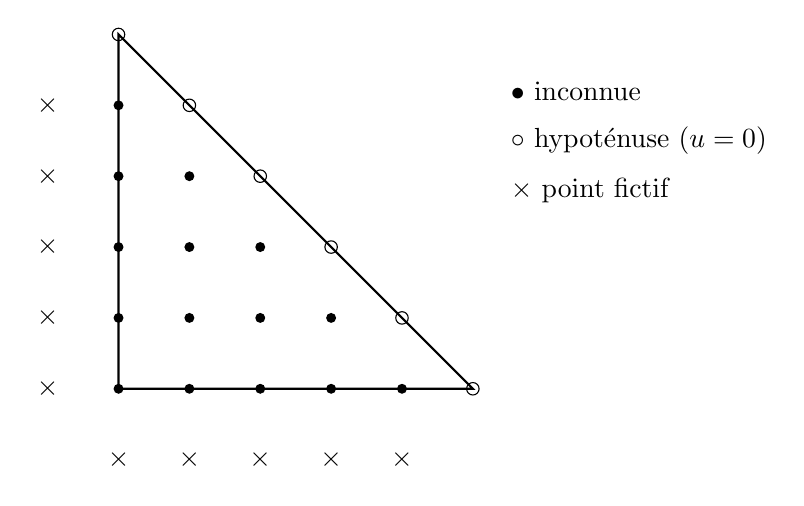
\begin{tikzpicture}[scale=0.9]
  \foreach \i in {0,...,5} \foreach \j in {0,...,5} {
    \pgfmathtruncatemacro{\s}{\i+\j}
    \ifnum\s<5 \fill (\i,\j) circle (2pt); \fi
    \ifnum\s=5 \draw (\i,\j) circle (2.5pt); \fi
  }
  \foreach \j in {0,...,4} \draw (-1,\j) node {$\times$};
  \foreach \i in {0,...,4} \draw (\i,-1) node {$\times$};
  \draw[thick] (0,0) -- (5,0) -- (0,5) -- cycle;
  \node[right] at (5.4,4.2) {$\bullet$ inconnue};
  \node[right] at (5.4,3.5) {$\circ$ hypoténuse ($u = 0$)};
  \node[right] at (5.4,2.8) {$\times$ point fictif};
\end{tikzpicture}
\end{center}

\Question{2)- Algorithme.}
\begin{algo}[ : Gauss-Seidel sur le triangle]
  \Require $l$, $h$, $a$, $N$, $\varepsilon$
  \State $\Delta x \leftarrow l/N$ ; $\Delta y \leftarrow h/N$ ; $\rho^2 \leftarrow (\Delta x/\Delta y)^2$
  \State $u_{i,j} \leftarrow 0$ pour $i + j \le N$
  \Repeat
    \State $\mathit{num} \leftarrow 0$ ; $\mathit{den} \leftarrow 0$
    \For{$i$ allant de $0$ à $N-1$}
      \For{$j$ allant de $0$ à $N-1-i$}
        \State $u_O \leftarrow u_{i-1,j}$ si $i > 0$, sinon $u_{1,j} + 2a\Delta x$
        \State $u_S \leftarrow u_{i,j-1}$ si $j > 0$, sinon $u_{i,1} + 2a\Delta y$
        \State $t \leftarrow \bigl[u_{i+1,j} + u_O + \rho^2(u_{i,j+1} + u_S)\bigr]/\bigl(2(1+\rho^2)\bigr)$
        \State $\mathit{num} \leftarrow \mathit{num} + \abs{t - u_{i,j}}$ ; $\mathit{den} \leftarrow \mathit{den} + \abs{t}$ ; $u_{i,j} \leftarrow t$
      \EndFor
    \EndFor
  \Until{$\mathit{num}/\mathit{den} < \varepsilon$}
  \Print $u_{i,j}$
\end{algo}
(Les valeurs $u_{i+1,j}$ et $u_{i,j+1}$ utilisées au voisinage de l'hypoténuse
sont les zéros imposés.)

\Verif Pour $l = h$, la fonction $u = a(l - x - y)$ est harmonique, nulle sur
l'hypoténuse, et vérifie $-\partial u/\partial y = -\partial u/\partial x = a$ :
c'est la solution exacte. Avec $a = 2$, $l = h = 1$, $N = 10$, l'algorithme
la retrouve à $4\times 10^{-12}$ près (543 itérations), ce qui valide le
traitement des points fictifs. (Pour $l \ne h$, il n'existe pas de solution
affine, mais l'algorithme est le même.)

\Refs Cours, chapitre VI (conditions de Neumann, formule (P4)) ;
\BF{§~12.1, alg.~12.1, p.~738--739}.
